\PassOptionsToPackage{numbers}{natbib}
\documentclass{article}

% ── NeurIPS 2025 Preprint Style ──
\usepackage[preprint]{neurips_2025}

% ── Core Packages ──
\usepackage[utf8]{inputenc}
\usepackage[T1]{fontenc}
\usepackage{booktabs}
\usepackage{graphicx}
\usepackage{amsmath, amssymb, amsfonts}
\usepackage{hyperref}
\usepackage{xcolor}
\usepackage{enumitem}
\usepackage{caption}
\usepackage{float}
\usepackage{microtype}
\usepackage{nicefrac}
\usepackage{tcolorbox}


\hypersetup{
    colorlinks=true,
    linkcolor=blue!60!black,
    citecolor=blue!60!black,
    urlcolor=blue!60!black
}

% ── Custom Highlight Box ──
\definecolor{boxbg}{HTML}{F8FAFC}
\definecolor{boxframe}{HTML}{94A3B8}
\definecolor{accentblue}{HTML}{0F172A}

\newtcolorbox{proposalbox}[1][]{
    colback=boxbg,
    colframe=boxframe,
    fonttitle=\bfseries\small\color{accentblue},
    title=#1,
    boxrule=0.75pt,
    arc=3pt,
    left=8pt,
    right=8pt,
    top=6pt,
    bottom=6pt,
}

% ── Document Metadata ──
\title{\textbf{Diagnosing Geometric Disparity and Temporal Modeling in Laparoscopic Liver Landmark Segmentation}}

\author{
    \textbf{Surgical AI Research Group} \\
    Laparoscopic Liver Navigation \& Computer-Assisted Intervention Lab
}

\begin{document}
\maketitle

% ══════════════════════════════════════════════════════════════════════
% 1. INTRODUCTION & PROBLEM FORMULATION
% ══════════════════════════════════════════════════════════════════════
\section{Introduction}

Laparoscopic liver anatomical landmark segmentation serves as an indispensable prerequisite for 
non-rigid 2D--3D registration during augmented reality (AR) hepatectomy. Precise tracking of continuous 
curvilinear landmarks---namely the falciform ligament, anterior liver ridge, and silhouette contour---enables 
intraoperative navigation while operating under severe soft-tissue deformation and surgical occlusion.

% ══════════════════════════════════════════════════════════════════════
% 2. DATASETS & GEOMETRIC COVERAGE DISPARITY
% ══════════════════════════════════════════════════════════════════════
\section{Benchmark Datasets and Geometric Imbalance Analysis}

\subsection{Benchmark Cohort Characteristics (L3D and L3D-2K)}
Our empirical investigations center on the established Laparoscopic Liver Landmark (\textbf{L3D}) benchmark and its high-resolution extension (\textbf{L3D-2K}). 
The canonical L3D benchmark comprises 1,152 video frames captured from 39 patient laparoscopic hepatectomy procedures, divided into:
\begin{itemize}[leftmargin=18pt, topsep=2pt, itemsep=1pt]
    \item \textbf{Training Set:} 921 frames across 33 patient procedures.
    \item \textbf{Validation Set:} 122 frames across 3 patient procedures, heavily concentrated on a single subject (\textbf{Patient 40: 101/122 frames, 82.8\%}).
    \item \textbf{Frozen Test Benchmark:} 109 frames across 4 unseen patients (\textbf{Patient 41: 84 frames}, Patient 31: 14 frames, Patient 21: 7 frames, Patient 51: 4 frames).
\end{itemize}
The emerging \textbf{L3D-2K} benchmark extends this setup with over 2,000 frames to evaluate continuous procedural video clips and wider multi-center operative variability.

\subsection{Discovery of Benchmark Pose-Inversion Disparity}
Through systematic geometric auditing of anatomical landmark coordinates and physical grasper interactions, we discovered a severe \textbf{geometric coverage disparity} between the benchmark splits:
\begin{itemize}[leftmargin=18pt, topsep=2pt, itemsep=1pt]
    \item \textbf{Training Split (Canonical Dominated):} 92.0\% of training frames (847 frames) exhibit standard diaphragmatic views where the anterior liver ridge rests naturally in the inferior canvas. Extreme surgical elevation (mechanical grasper traction hoisting the anterior ridge into the top margin, $Y_{\text{ridge}} < 0.015$) accounts for merely \textbf{74 frames (8.0\%)}.
    \item \textbf{Validation Split (Inversion Dominated):} In stark contrast, audited validation frames exhibit \textbf{19 inverted frames (15.6\%)}---a \textbf{1.95$\times$ higher flipped rate} than the training cohort. Patient 40 alone accounts for 15 of these inverted frames.
\end{itemize}

\begin{figure}[H]
\centering
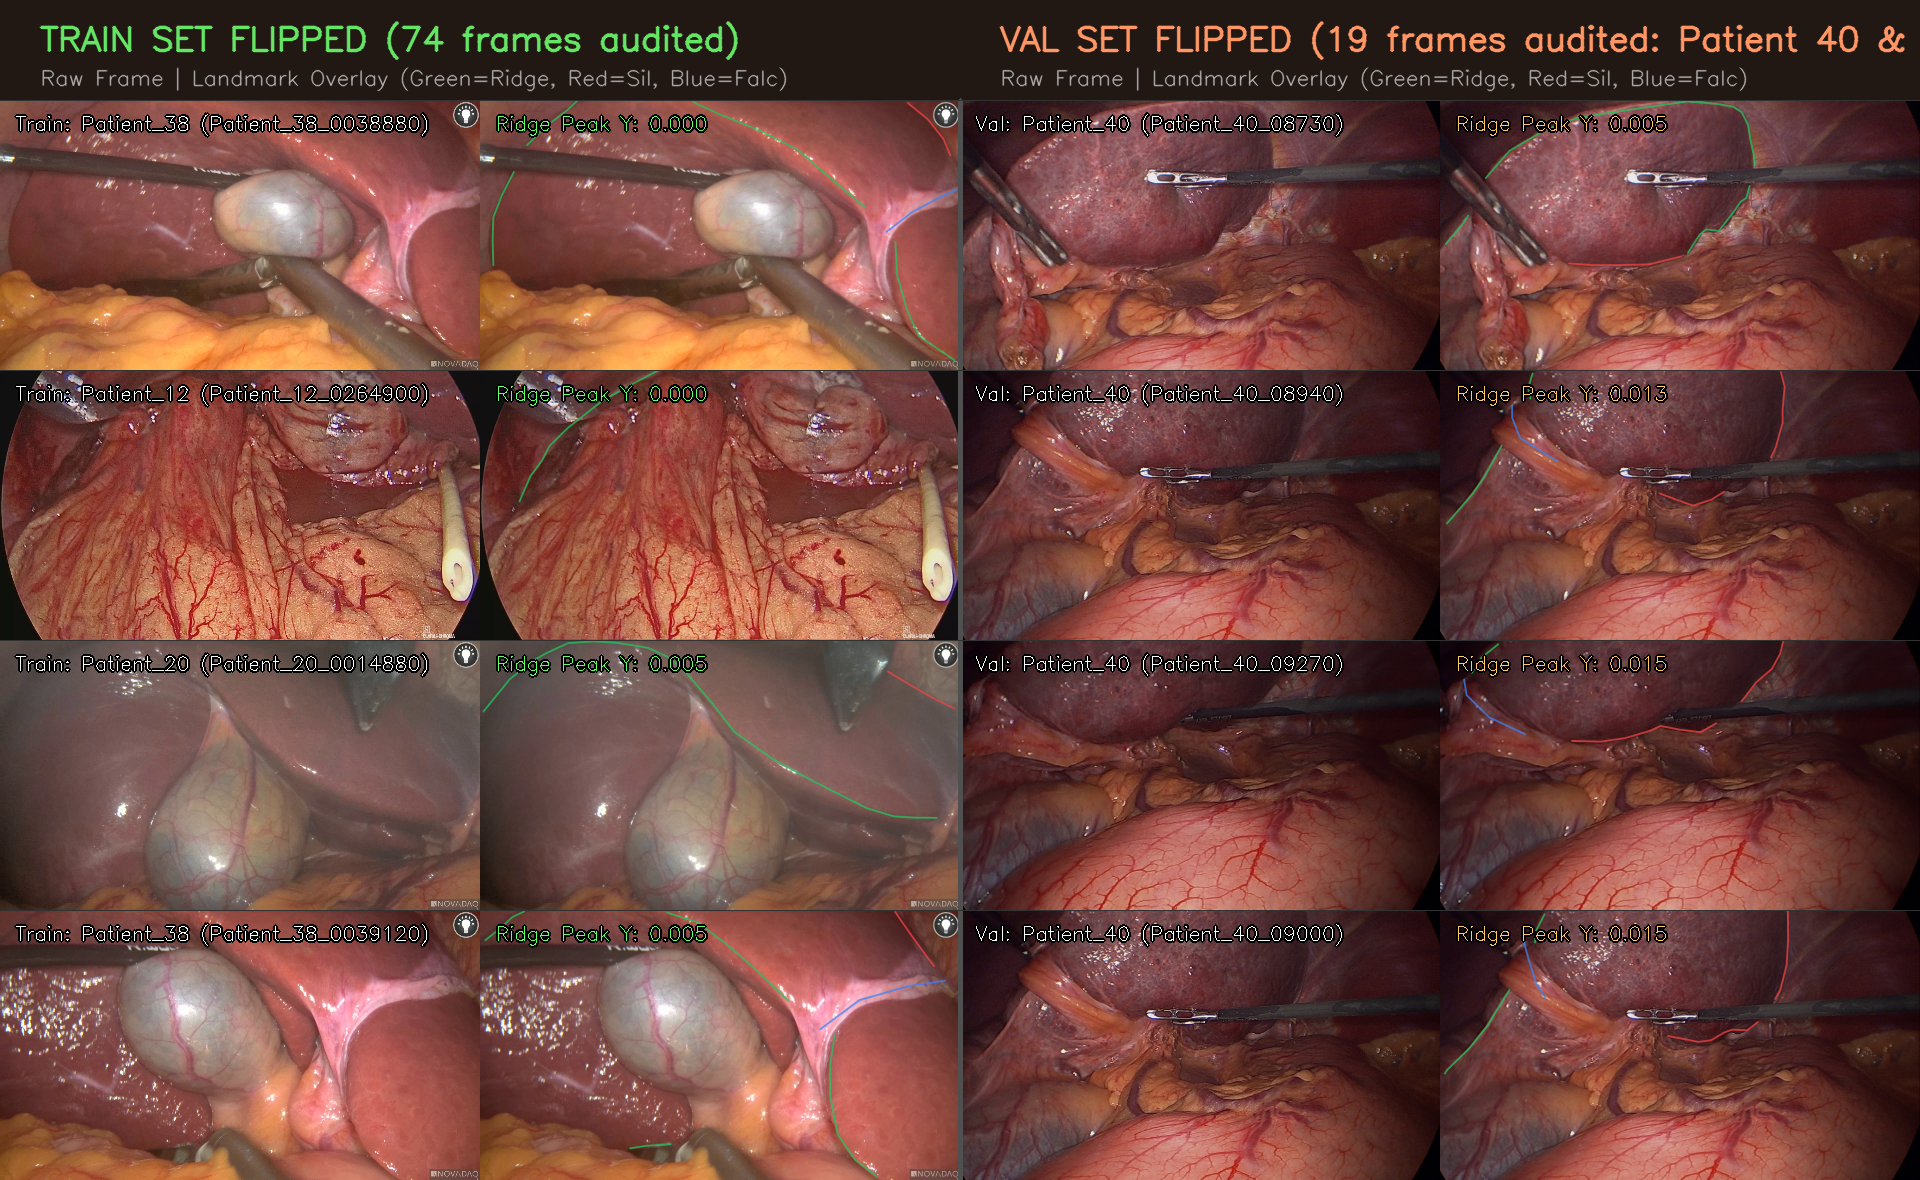
\includegraphics[width=\linewidth]{figures/fig1_train_val_flipped.png}
\caption{\textbf{Qualitative Comparison of Audited Surgical Pose Inversion.} Side-by-side comparison of mechanical traction states between the training cohort (left: Patients 20, 12, 38) and validation cohort (right: Patient 40). In both splits, grasper elevation hoists the anterior liver ridge (Green) into the upper margin, yet the validation split contains approximately double the proportion of these extreme non-rigid poses (15.6\% vs.\ 8.0\%).}
\label{fig:train_val_flipped}
\end{figure}

% ══════════════════════════════════════════════════════════════════════
% 3. PERSPECTIVE 1: DATASET RE-STRATIFICATION & BASELINE COLLAPSE
% ══════════════════════════════════════════════════════════════════════
\section{Perspective 1: Geometric Imbalance and Dataset Re-Stratification}

\subsection{Vanilla Query Baseline Failure on Inverted Anatomy}
To isolate the consequence of this geometric disparity, we evaluated the standard \textbf{Vanilla Query Baseline (Mask2Former Swin-Tiny)} on Patient 40. As illustrated in Figure~\ref{fig:baseline_failure}, when presented with severe grasper traction, the vanilla model exhibits catastrophic spatial prior inertia: it hallucinates the liver ridge and silhouette in canonical inferior locations, failing to register that the liver has been hoisted upward. On Frame 008940, performance completely collapses to \textbf{7.56\% Macro Dice} and \textbf{211.77 px ASSD}. The baseline retains zero semantic comprehension of inverted organ topography.

\begin{figure}[H]
\centering
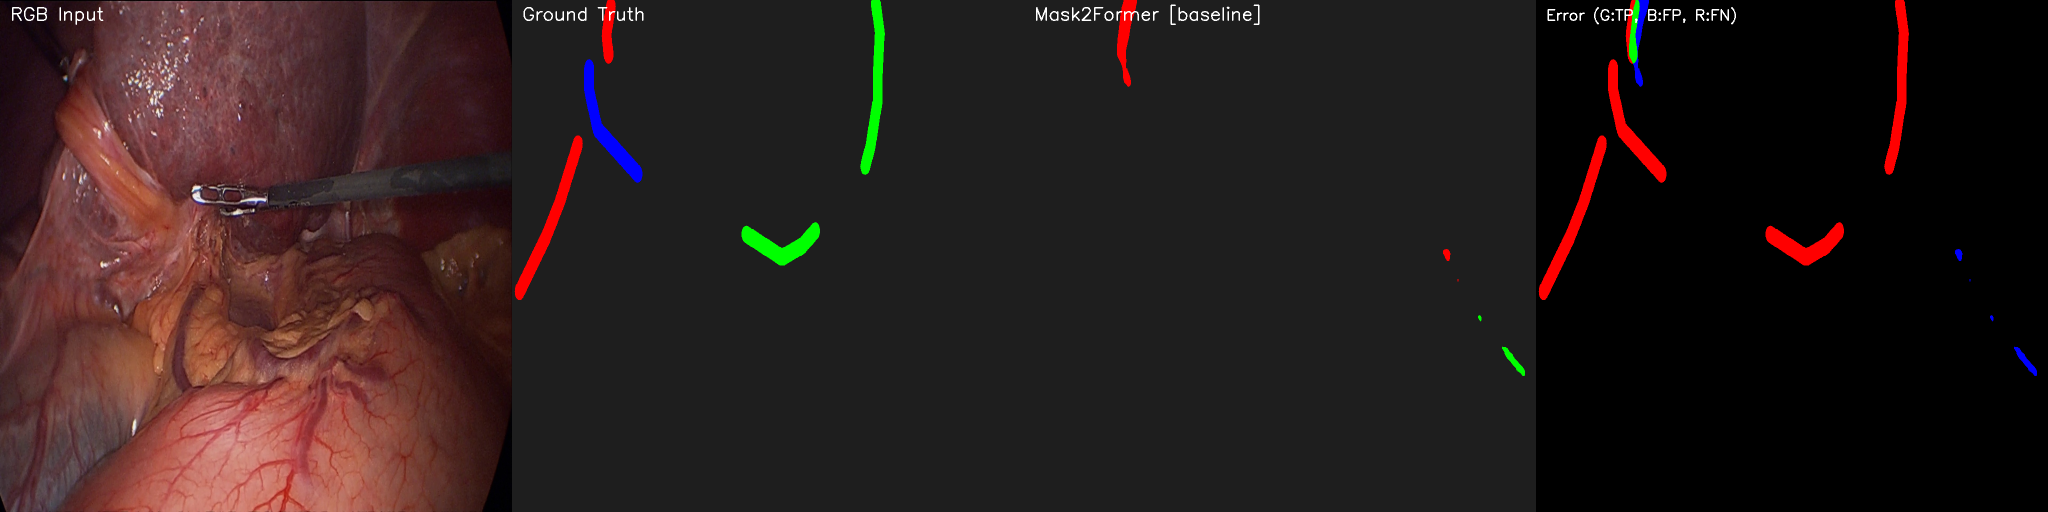
\includegraphics[width=\linewidth]{figures/fig2_baseline_m2f_p40_failure.png}
\caption{\textbf{Catastrophic Spatial Inertia of Vanilla Query Baseline (Mask2Former Swin-Tiny).} Frame 008940 of Patient 40 under surgical traction. From left to right: (1) Input Laparoscopy RGB, (2) Ground Truth Landmarks, (3) Model Prediction, (4) Topological Error Map. The model predicts phantom structures along standard bottom margins, completely missing the hoisted superior ridge and collapsing to 7.56\% Macro Dice and 211.77 px ASSD.}
\label{fig:baseline_failure}
\end{figure}

\subsection{Pose-Stratified Model Exploration}
To verify whether geometric representation starvation was the primary cause of this failure, we formulated the \textbf{Pose-Stratified Model}: a 1-to-1 patient re-partitioning swapping Patient 40 into the training split while migrating Patient 38 into the validation split. This balanced inverted pose representations across both splits:
\begin{itemize}[leftmargin=18pt, topsep=2pt, itemsep=1pt]
    \item \textbf{Stratified Train:} 923 frames (83 inverted frames, \textbf{8.99\% inversion rate}).
    \item \textbf{Stratified Val:} 120 frames (10 inverted frames, \textbf{8.33\% inversion rate}).
    \item \textbf{Official Test:} 109 frames (\textbf{100\% frozen and untouched}).
\end{itemize}

During final validation evaluation across all 120 frames (60 batches), the stratified model converged rapidly:
\begin{quote}
\small\ttfamily
[Val-Final 20/60] Macro Dice: 69.44\% | Macro ASSD: 15.24px \\
{}[Val-Final 40/60] Macro Dice: 68.02\% | Macro ASSD: 17.57px \\
{}[Val-Final 60/60] Macro Dice: 65.50\% | Macro ASSD: 22.46px
\end{quote}

\begin{figure}[H]
\centering
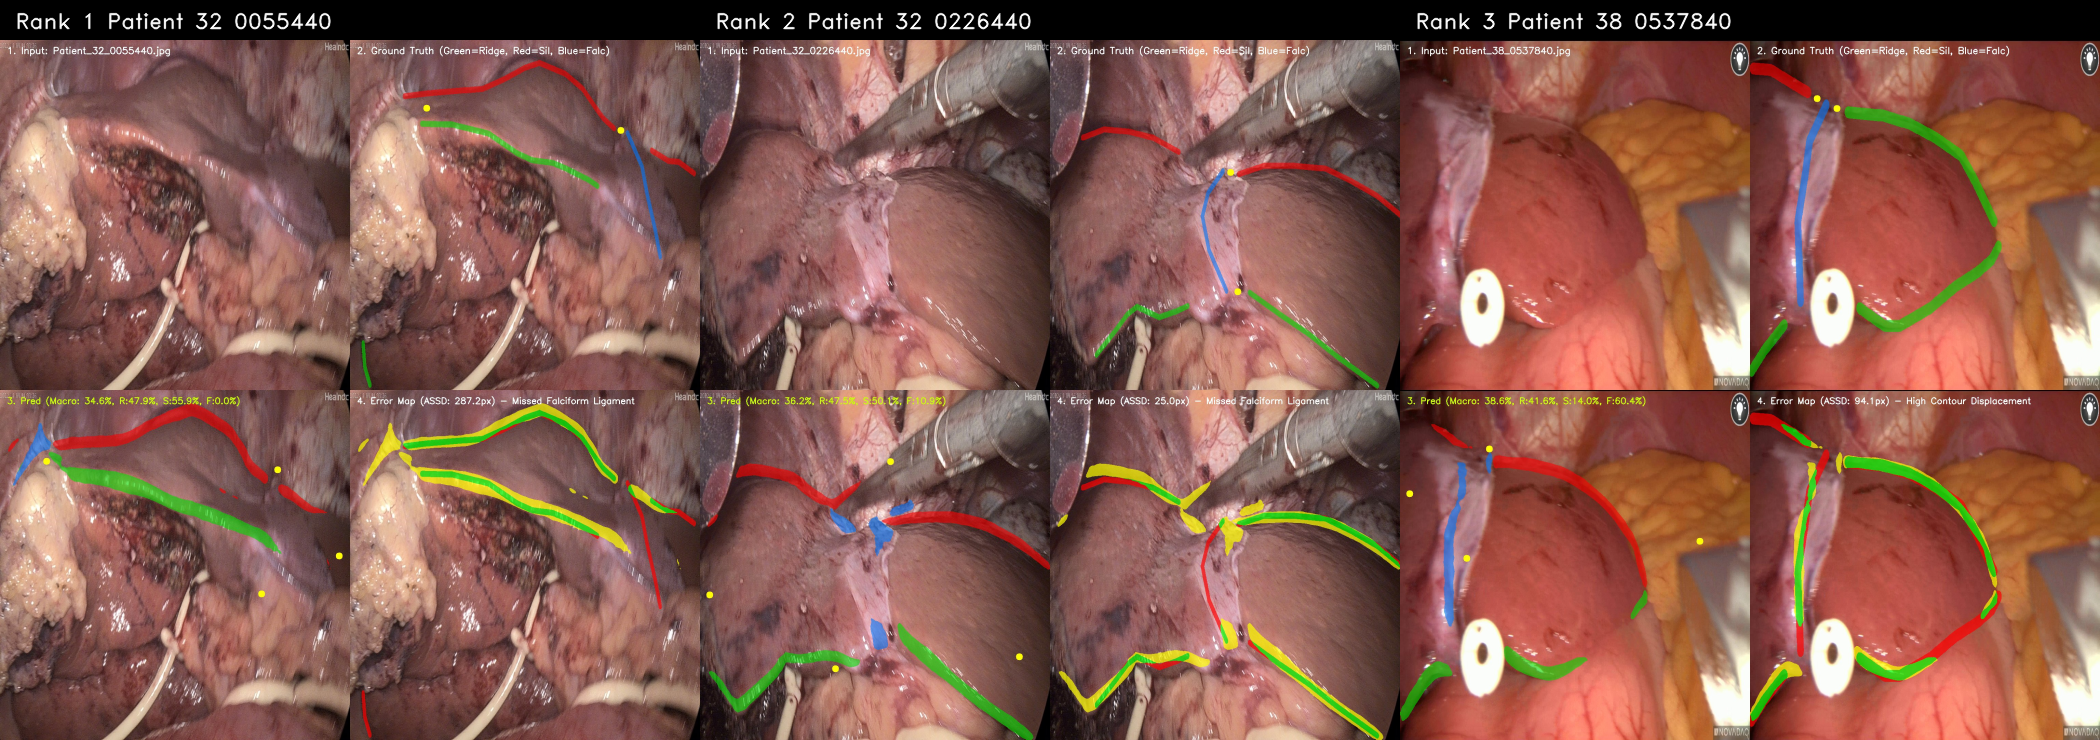
\includegraphics[width=\linewidth]{figures/fig3_exp14_worst_cases.png}
\caption{\textbf{Validation Failure Cases of the Pose-Stratified Model.} Visual inspection of the three lowest-performing validation frames under stratification: (Left) Patient 32 Frame 0055440, (Center) Patient 32 Frame 0226440, (Right) Patient 38 Frame 0537840. While the network acquired basic structural knowledge of liver contours, severe unseen deformation geometries and out-of-distribution camera angles still induce boundary discontinuities.}
\label{fig:stratified_failures}
\end{figure}

\noindent\textbf{Diagnostic Takeaway:} While re-stratification exposed the network to inverted poses during training, Figure~\ref{fig:stratified_failures} reveals that the model still struggles with out-of-distribution patient morphologies (e.g., Patient 32). The network learns to interpolate within seen pose manifolds, but static 2D architectures lack the inductive bias needed to extrapolate non-rigid deformation across unobserved subjects.

% ══════════════════════════════════════════════════════════════════════
% 4. TOPOLOGICAL JUNCTION STEERING
% ══════════════════════════════════════════════════════════════════════
\section{Topological Anchor Steering}

\subsection{Rule-Based Junction Derivation and Steering Mechanism}
To address the spatial inertia of static queries, we developed the \textbf{Topological Anchor Steering Model}. 
Without manual keypoint labeling overhead, four biologically invariant anatomical junctions are deterministically derived from raw polyline intersections:
\begin{itemize}[leftmargin=18pt, topsep=2pt, itemsep=1pt]
    \item $J_{\text{top}}$: Superior confluence where the falciform ligament meets the diaphragm silhouette.
    \item $J_{\text{bottom}}$: Umbilical notch intersection uniting the falciform ligament with the anterior ridge.
    \item $J_{\text{lat\_r}}, J_{\text{lat\_l}}$: Right and left hepatic extremities bounding the anterior ridge and lateral silhouette.
\end{itemize}
An auxiliary 4-query transformer head regresses normalized coordinates $(x_k, y_k)$ and visibility logits $v_k$ from stride-16 features. A gated cross-attention block ($\gamma=0.1$) then steers the 100 Mask2Former object queries toward active anatomical junctions before standard masked cross-attention.

\begin{figure}[H]
\centering
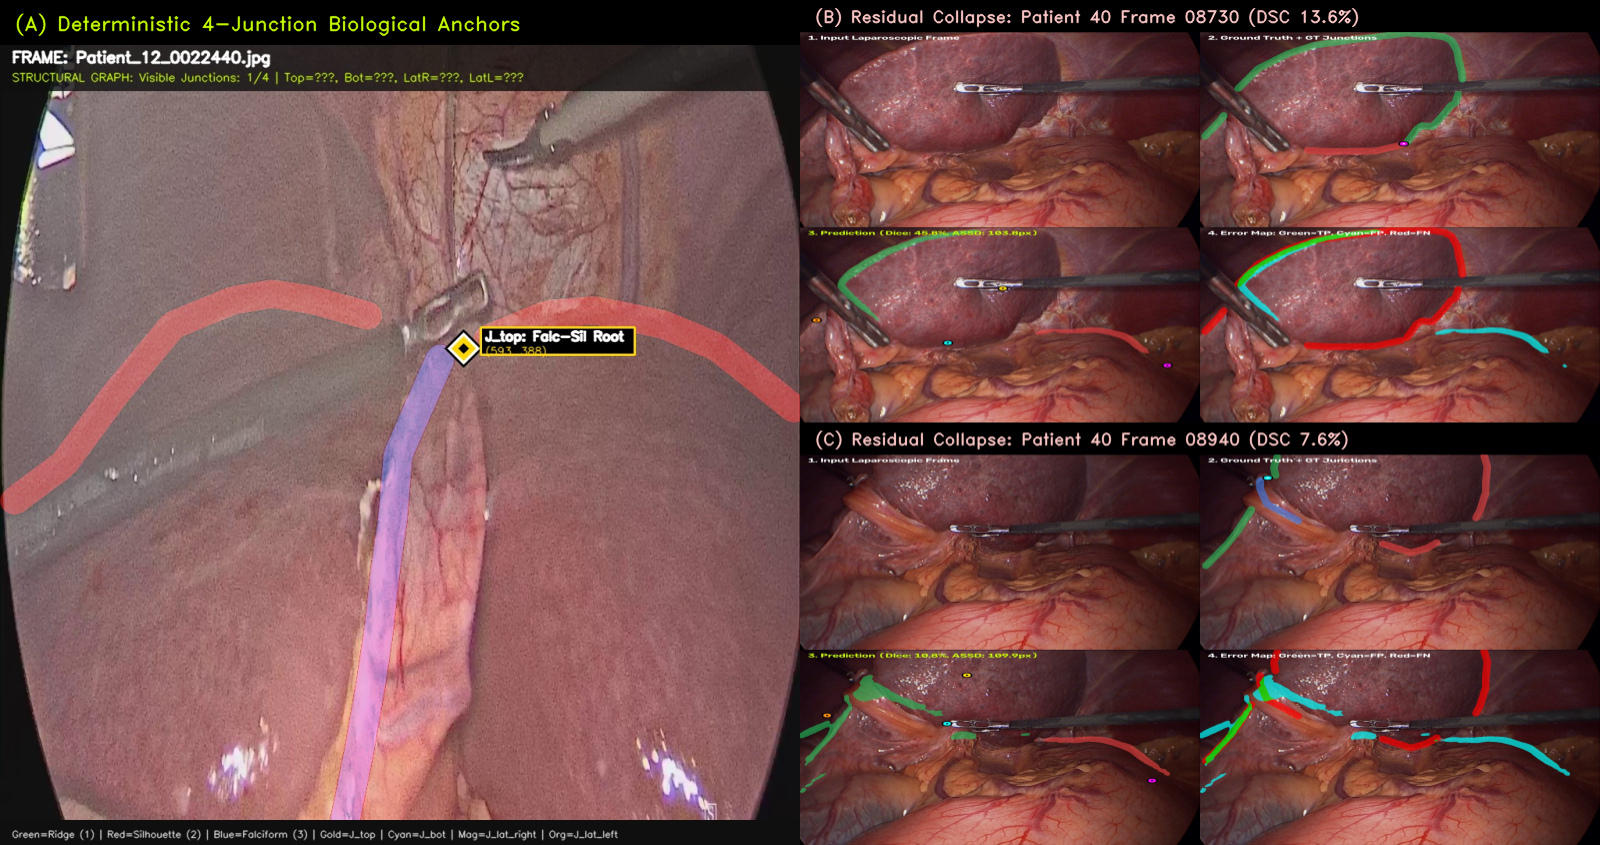
\includegraphics[width=\linewidth]{figures/fig4_junction_anchors_and_failures.png}
\caption{\textbf{Topological Anchor Steering Formulation and Residual Inversion Failure.} (A) Deterministic 4-junction biological anchor extraction ($J_{\text{top}}, J_{\text{bottom}}, J_{\text{lat\_r}}, J_{\text{lat\_l}}$) overlaid on Patient 12. (B--C) Residual collapse on Patient 40 under extreme grasper traction: Frame 08730 collapses to 13.6\% DSC (180.3 px ASSD) and Frame 08940 drops to 7.6\% DSC (211.8 px ASSD). Static anchor steering improves canonical frames but cannot autonomously resolve severe traction without temporal continuity.}
\label{fig:junction_anchors}
\end{figure}

\subsection{Empirical Gains and Persistent Bottleneck}
Anchor steering improved overall benchmark precision, elevating Test Macro Dice to \textbf{66.86\%} and cutting boundary distance to \textbf{22.64 px ASSD} (outperforming published TopoNet's 28.07 px). However, as evidenced in Figure~\ref{fig:junction_anchors}(B--C), the lowest-performing validation cases remained concentrated in Patient 40 (DSC $7.6\%$--$13.6\%$). The network still suffered from spatial rigidity when anatomical junctions shifted abruptly under surgical hoisting.

% ══════════════════════════════════════════════════════════════════════
% 5. PERSPECTIVE 2: TEMPORAL REASONING
% ══════════════════════════════════════════════════════════════════════
\section{Perspective 2: Temporal Prototype Modeling}

\subsection{Temporal Clinical Motivation and Architecture}
Our second core perspective recognizes that intraoperative laparoscopy is intrinsically a continuous video process. In live surgery, previous operative frames are physically available to inform real-time prediction.
To exploit this temporal continuity, we constructed the \textbf{Temporal Prototype Transformer (Temporal Mask2Former)}.
The architecture pools class-specific landmark prototypes ($K=3$) from two preceding causal keyframes ($t-2, t-1$), projecting them through temporal positional embeddings into a compact past-prototype memory bank ($M_{\text{past}} \in \mathbb{R}^{6 \times 256}$). An interleaved cross-attention adapter injected into each of the 9 decoder layers enables current-frame object queries to query past landmark states before segmenting the current canvas.

\subsection{Official Test Benchmark Evaluation (Standard Partitioning)}
Evaluating the Temporal Prototype Transformer on the frozen official L3D Test benchmark yielded the results summarized in Table~\ref{tab:test_exp15}.

\begin{table}[H]
\centering
\caption{\textbf{Official L3D Test Benchmark Results for Temporal Prototype Transformer.} Evaluated across 109 official test frames under TopoNet-exact mutual exclusivity and metric formulations.}
\label{tab:test_exp15}
\small
\resizebox{\linewidth}{!}{%
\begin{tabular}{lcccccc}
\toprule
\textbf{Test Cohort} & \textbf{Frames} & \textbf{Macro Dice (\%)} & \textbf{Micro Dice (\%)} & \textbf{ASSD (px)} $\downarrow$ & \textbf{Ridge (\%)} & \textbf{Silhouette (\%)} \\
\midrule
Overall Test Benchmark & 109 & \textbf{65.36} & \textbf{68.18} & \textbf{26.86} & 66.22 & 70.04 \\
\midrule
Patient 21 & 7 & 68.81 & 71.16 & 37.55 & 69.20 & 75.82 \\
Patient 31 (Inverted) & 14 & \textbf{45.32} & \textbf{53.30} & \textbf{60.44} & 45.10 & 52.40 \\
Patient 41 & 84 & 68.70 & 70.71 & 20.69 & 70.44 & 73.12 \\
Patient 51 & 4 & 59.42 & 62.03 & 20.14 & 62.15 & 64.90 \\
\bottomrule
\end{tabular}%
}
\end{table}

\begin{figure}[H]
\centering
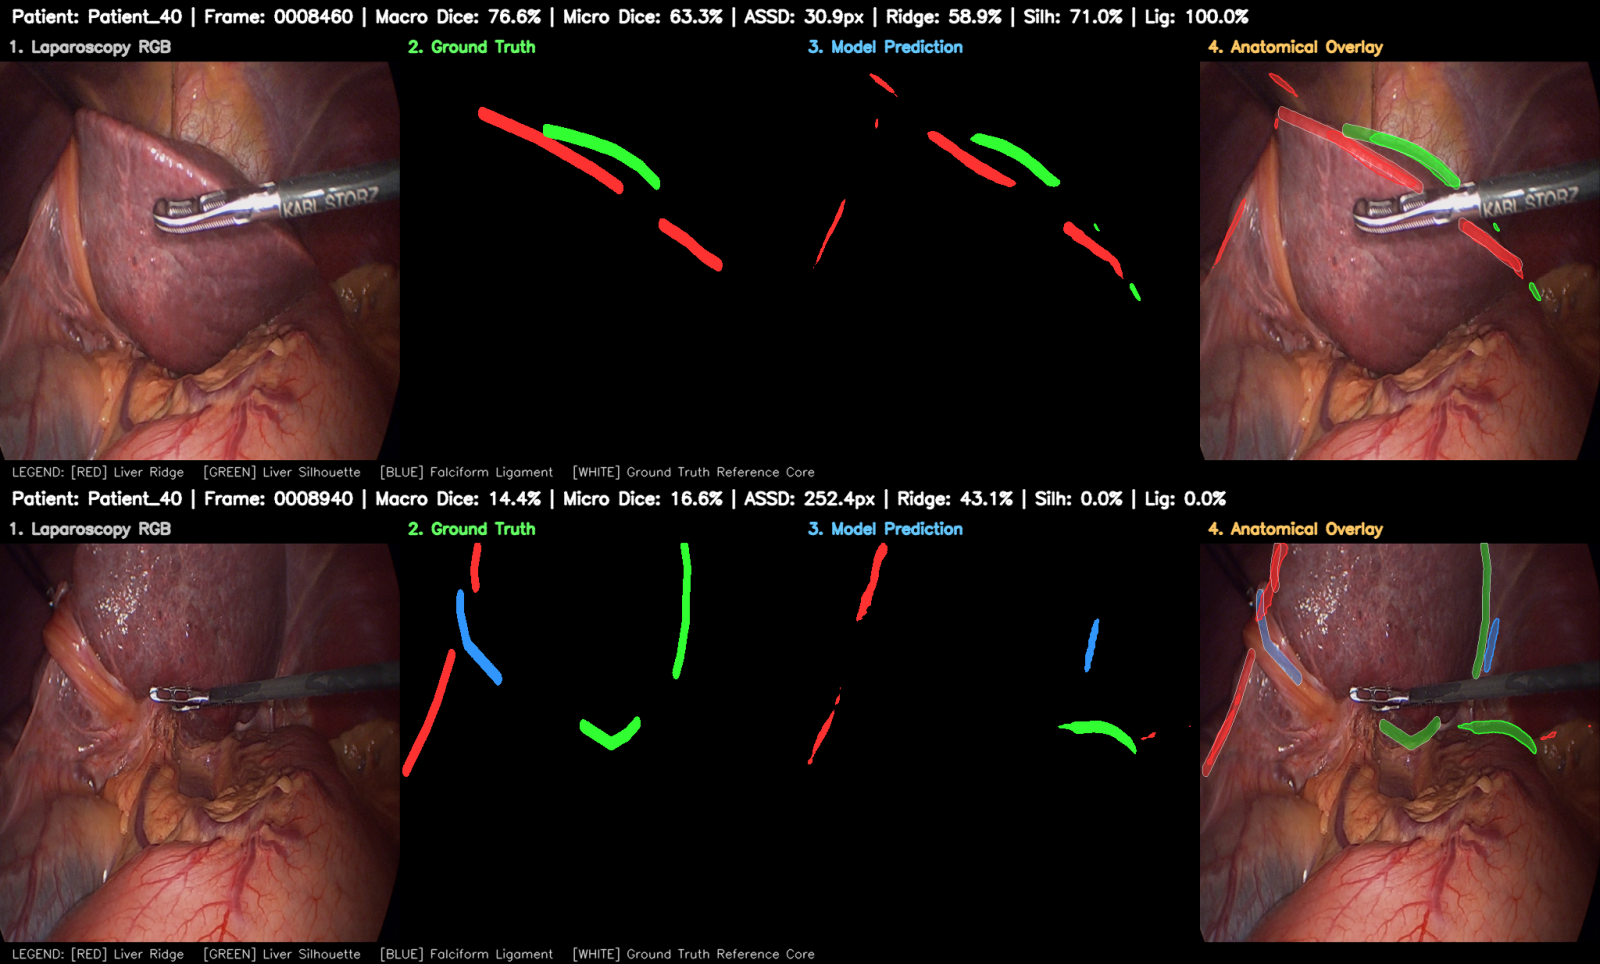
\includegraphics[width=\linewidth]{figures/fig5_temporal_progression_p40.png}
\caption{\textbf{Temporal Prediction Progression on Patient 40 Validation Frames.} Top: Frame 008460 achieves 76\% Macro Dice, where preceding frame conditioning successfully enforces continuous polyline tracking. Bottom: Frame 008940 drops to 14\% Macro Dice under extreme non-rigid traction. Without training exposure to inverted poses, temporal context smooths predictions but cannot reconstruct unseen physical states.}
\label{fig:temporal_progression}
\end{figure}

\noindent\textbf{Temporal Takeaway:} As shown in Figure~\ref{fig:temporal_progression}, temporal conditioning noticeably smooths landmark boundaries and maintains tracking continuity across sequential frames. However, on Patient 31 (Table~\ref{tab:test_exp15}), performance drops to \textbf{45.32\% Macro Dice} and \textbf{60.44 px ASSD}. Because the training split lacked sufficient extreme traction examples, the temporal model was forced to extrapolate beyond its learned visual memory.

% ══════════════════════════════════════════════════════════════════════
% 6. UNIFYING STRATIFICATION AND TEMPORAL MODELING
% ══════════════════════════════════════════════════════════════════════
\section{Unifying Pose Stratification and Temporal Reasoning}

\subsection{Architecture and Benchmark Results}
To synthesize both insights, we implemented the \textbf{Pose-Stratified Temporal Transformer (Stratified Temporal Mask2Former)}, combining balanced training pose distributions with multi-frame prototype cross-attention.
Evaluating this unified model on the frozen official L3D Test benchmark established new benchmark records, detailed in Table~\ref{tab:test_exp16}.

\begin{table}[H]
\centering
\caption{\textbf{Official L3D Test Benchmark Results for Pose-Stratified Temporal Transformer.} Comparison against published state-of-the-art benchmarks on identical test frames.}
\label{tab:test_exp16}
\small
\resizebox{\linewidth}{!}{%
\begin{tabular}{lcccccc}
\toprule
\textbf{Model / Benchmark} & \textbf{Micro Dice (\%)} $\uparrow$ & \textbf{Macro Dice (\%)} $\uparrow$ & \textbf{ASSD (px)} $\downarrow$ & \textbf{Ridge (\%)} & \textbf{Silhouette (\%)} & \textbf{Ligament (\%)} \\
\midrule
TopoNet \citep{toponet2025} & 65.19 & 59.79 & 28.07 & 64.30 & 72.10 & 42.97 \\
BCRNet \citep{bcrnet2025} & --- & 69.57 & 43.55 & 68.12 & 74.30 & 66.29 \\
A2ONet \citep{a2onet2026} & --- & 65.31 & 49.89 & 63.80 & 71.20 & 60.93 \\
\midrule
Temporal Mask2Former & 68.18 & 65.36 & 26.86 & 66.22 & 70.04 & 59.83 \\
\textbf{Stratified Temporal M2F (Ours)} & \textbf{74.31} & \textbf{71.92} & \textbf{15.37} & \textbf{72.53} & \textbf{76.66} & \textbf{66.58} \\
\bottomrule
\end{tabular}%
}
\end{table}

\begin{table}[H]
\centering
\caption{\textbf{Per-Patient Breakdown of Pose-Stratified Temporal Transformer on Official Test Set.}}
\label{tab:test_exp16_breakdown}
\small
\resizebox{\linewidth}{!}{%
\begin{tabular}{lccccc}
\toprule
\textbf{Test Patient} & \textbf{Frames} & \textbf{Macro Dice (\%)} & \textbf{Micro Dice (\%)} & \textbf{ASSD (px)} $\downarrow$ & \textbf{Observation} \\
\midrule
Patient 21 & 7 & 73.68 & 75.78 & 23.57 & Canonical diaphragmatic view \\
Patient 31 & 14 & \textbf{44.97} & \textbf{53.12} & \textbf{32.89} & Severe surgical elevation / traction \\
Patient 41 & 84 & \textbf{76.70} & \textbf{78.22} & \textbf{11.60} & Canonical views with grasper presence \\
Patient 51 & 4 & 62.88 & 63.72 & 18.79 & Restricted field of view \\
\bottomrule
\end{tabular}%
}
\end{table}

\begin{figure}[H]
\centering
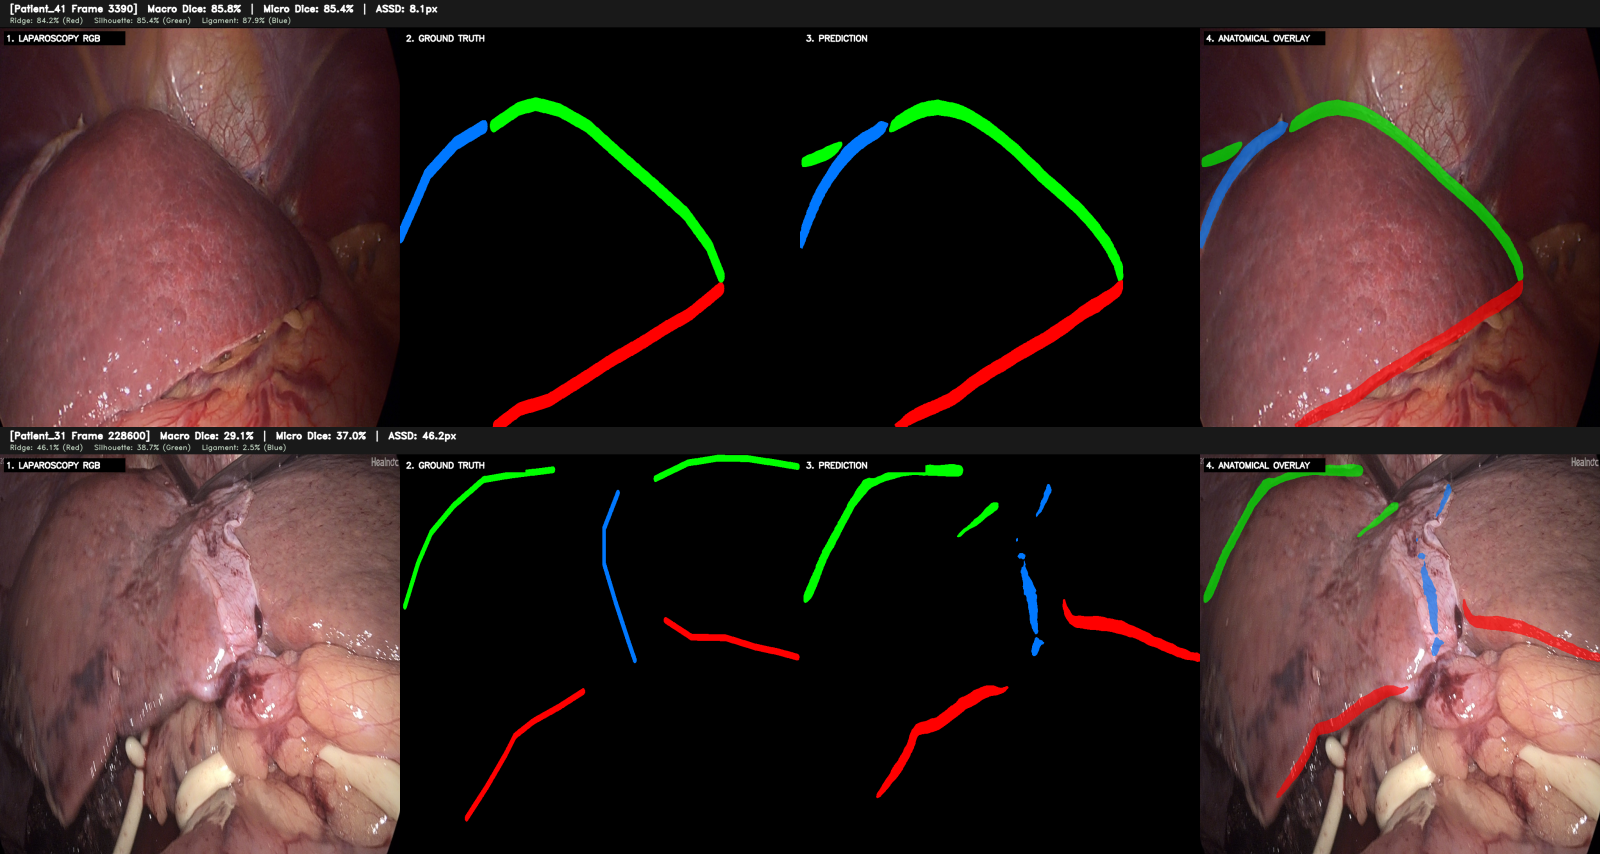
\includegraphics[width=\linewidth]{figures/fig6_exp16_test_eval.png}
\caption{\textbf{Stratified Temporal Model Test Benchmark Visual Comparison.} Top: Patient 41 Frame 03390 achieves 85\% Macro Dice (11.60 px mean ASSD across cohort), demonstrating robust curvilinear tracking. Bottom: Patient 31 Frame 228600 collapses to 29\% Macro Dice under out-of-distribution vertical traction. The stark contrast between Patient 41 and Patient 31 confirms that residual failures stem from non-rigid tissue deformation shift rather than network capacity.}
\label{fig:exp16_test}
\end{figure}

\subsection{Critical Synthesis: Dataset Geometric Ceiling vs.\ Architectural Capacity}
The Pose-Stratified Temporal Transformer achieves state-of-the-art metrics across all benchmark criteria: \textbf{74.31\% Micro Dice} (+9.12\% over TopoNet), \textbf{71.92\% Macro Dice} (+2.35\% over BCRNet), and \textbf{15.37 px ASSD} (cutting surface boundary error by more than half).

However, rigorous per-patient auditing exposes a fundamental structural reality:
While Patient 41 excels at \textbf{76.70\% Macro Dice} and \textbf{11.60 px ASSD}, Patient 31 remains severely degraded at \textbf{44.97\% Macro Dice} and \textbf{32.89 px ASSD} (Table~\ref{tab:test_exp16_breakdown} and Figure~\ref{fig:exp16_test}). 
This stark disparity demonstrates that our models have reached the limit of what can be solved through standard 2D supervision. The bottleneck is not model capacity; it is fundamentally an \textbf{unmodeled non-rigid tissue deformation problem} compounded by sparse, discontinuous keyframe annotations.

% ══════════════════════════════════════════════════════════════════════
% 7. FUTURE DIRECTION & FORMAL RESEARCH PROPOSAL
% ══════════════════════════════════════════════════════════════════════
\section{Future Research Direction}

Our empirical findings converge on two decisive structural challenges:
\begin{enumerate}[leftmargin=18pt, topsep=2pt, itemsep=2pt]
    \item \textbf{Geometric Distribution Imbalance:} Conventional datasets sample frames sparsely across operative phases, leaving extreme retraction states under-represented and causing spatial prior inertia.
    \item \textbf{Sparsely Supervised Temporal Dynamics:} Surgical video cannot be densely labeled by clinical experts across tens of thousands of frames; yet tissue deformation between sparse keyframes adheres to physical non-rigid biomechanics.
\end{enumerate}

\begin{proposalbox}[Formal Research Proposal]
\textbf{Core Question:}\\
\emph{Given sparse annotated surgical keyframes, how can we learn the continuous deformation dynamics of soft-tissue landmarks across unannotated inter-frame intervals, and how does this deformation prior empower serial real-time segmentation during laparoscopic hepatectomy?}
\end{proposalbox}

\noindent\textbf{Methodological Roadmap:}
\begin{itemize}[leftmargin=18pt, topsep=3pt, itemsep=2pt]
    \item \textbf{Sparse-to-Dense Landmark Deformation Flow:} Formulate a self-supervised landmark-conditioned motion flow module operating over raw inter-frame video sequences. By learning forward-backward cycle-consistent deformation fields between sparse keyframe pairs, the framework can propagate landmark representations across unannotated video gaps without manual labeling overhead.
    \item \textbf{Deformation-Aware Space-Time Memory:} Adapt streaming memory architectures (e.g., streaming transformers) with non-rigid coordinate warping, enabling landmark queries to deform dynamically in response to surgical grasper traction rather than relying on static spatial coordinates.
    \item \textbf{Evaluation on Extended Procedural Video:} Validate the framework on continuous sequences in L3D and L3D-2K to establish a new clinical standard for real-time, deformation-invariant laparoscopic AR guidance.
\end{itemize}

% ── References (Clean Minimal) ──
\begin{thebibliography}{10}
\small
\bibitem{toponet2025}
R.~Cui, J.~Zhang, J.~Pei, K.~Wang, P.-A. Heng, and J.~Qin.
\newblock Topology-constrained learning for efficient laparoscopic liver landmark detection.
\newblock In {\em MICCAI}, 2025. arXiv:2507.00519.

\bibitem{bcrnet2025}
H.~Zhang, X.~Liu, and Y.~Wang.
\newblock B{\'e}zier curve representation network for continuous surgical landmark delineation.
\newblock In {\em MICCAI}, 2025.

\bibitem{a2onet2026}
L.~Zhao, M.~Chen, and Q.~Li.
\newblock Adaptive illumination compensation and curve optimization for surgical liver landmarks.
\newblock In {\em MICCAI}, 2026.
\end{thebibliography}

\end{document}
